
\section{Isocontour extraction}
If histograms provide statistical overviews of the range space of data, isocontour (isosurface)
extraction reveals data's structures and features of interest, such as objects or organs in medical
imaging, or a flame's front in combustion simulation. Sequences of isocontours can reveal important
topological structures in data. Extraction of isocontour is therefore an essential task in any
visualization and analysis system. In this section we study the characteristics of bit streams that
minimize errors in the reconstructed contour at all time.

As before, we begin by defining an error metric two compare two contours. A popular metric is the
Hausdorff distance [CITE] between two curves (in 2D) or two surfaces (in 3D), but we have found that
using the number of misclassified samples result is a more robust mertic. This metric can be
computed without actually extracting contours. Given two grid of values $G_1$ and $C_2$, and an
isovalue $v$, we classify each sample of each grid with a binary label, $0$ means the sample's value
is less than $v$, and $1$ means the opposite. Then, we perform an element-wise XOR of the resulting
two binary grids, and count the number of $1$'s in the result. This number is the number of samples
that were classified differently between the two grids, and in our experience, is a close proxy to
how different the two corresponding isocontours would be from each other.

Using just the number of misclassified voxels as the error metric in Algorithm [REF] is
insufficient, however. We have found that in step TODO of the algorithm, if the error caused by
switching off a chunk is too small (in orders of sub-pixel/sub-voxel), then the importance of the
chunk cannot be properly measured. We therefore amend the error metric by adding to it the relative
difference in length between two contours. This relative difference is, most of the time, a number
between $0$ and $1$,computed by the formula $|L(C_1)-L(C_2)|/L(C_1)$, where $L(C)$ is the length of
a contour $C$. The idea is that when the number number of misclassified voxels is less than $1$, the
error -- which is at the sub-pixel level -- is captured by the relative difference in contour length
instead.

With an error metric defined, we can compute an \emph{isocontour-optimized} stream for a data set,
given an isovalue. However, it is not straightforward to compare an \emph{isocontour-optimized}
stream to an \emph{rmse-optimized} stream in any contour error metric, because in practice, an
isocontour occupies an order of magnitude fewer grid cells, compared to the whole grid. An
\emph{rmse-optimized} stream has no reason to prioritize these cells, which is what an
\emph{isocontour-optimized} stream would do. In other words, the \emph{isocontour-optimized} stream
is spatially adaptive to a much higher degree than the \emph{rmse-optimized} stream is, and this
makes a direct comparison less meaningful. One way to solve this problem is to isolate the spatial
adaptivity aspect of a stream from its core characteristics (i.e., its tendency to favor precision
or resolution). Our solution is to divide space into regions, and study the relative order in which
a stream consumes bits within a region (in a way similar to how we construct a stream's signature),
while keeping the ordering of regions constant across streams.


\begin{figure}
	\centering
	\subcaptionbox{boiler}
	{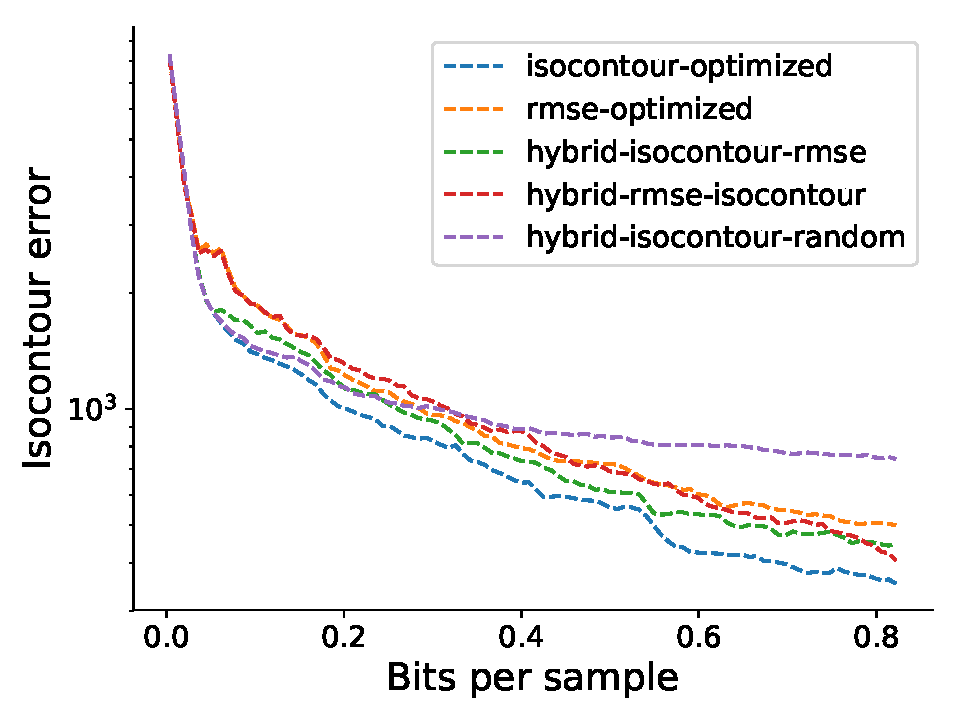
\includegraphics[width=0.48\linewidth]{img/isocontour/boiler-isocontour.pdf}}
	\subcaptionbox{boiler}
	{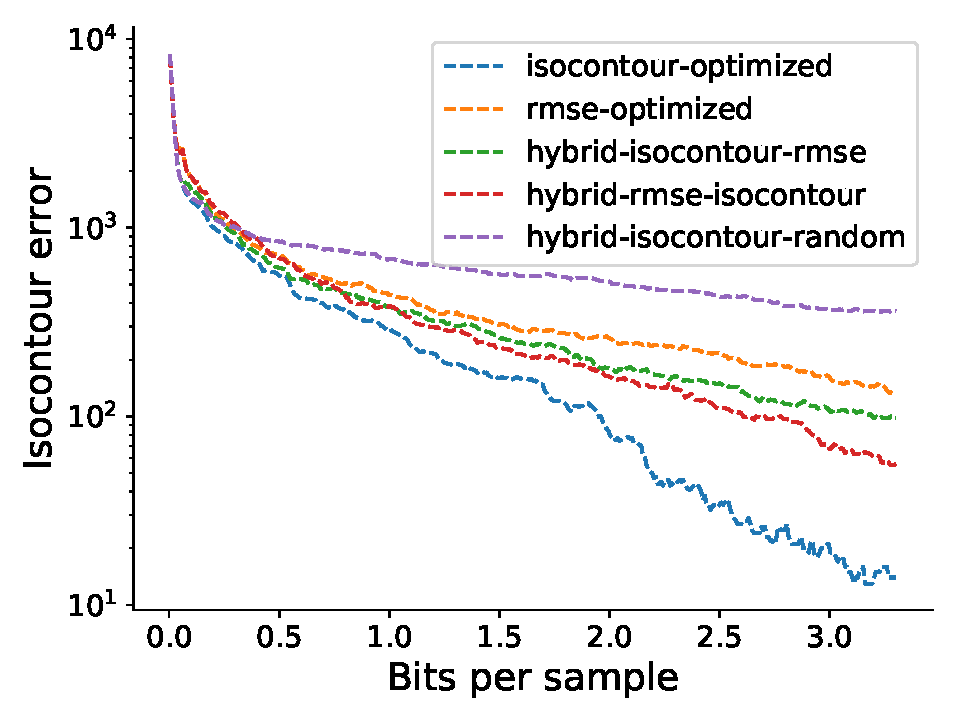
\includegraphics[width=0.48\linewidth]{img/isocontour/boiler-isocontour-long.pdf}}
	\subcaptionbox{kingsnake}
	{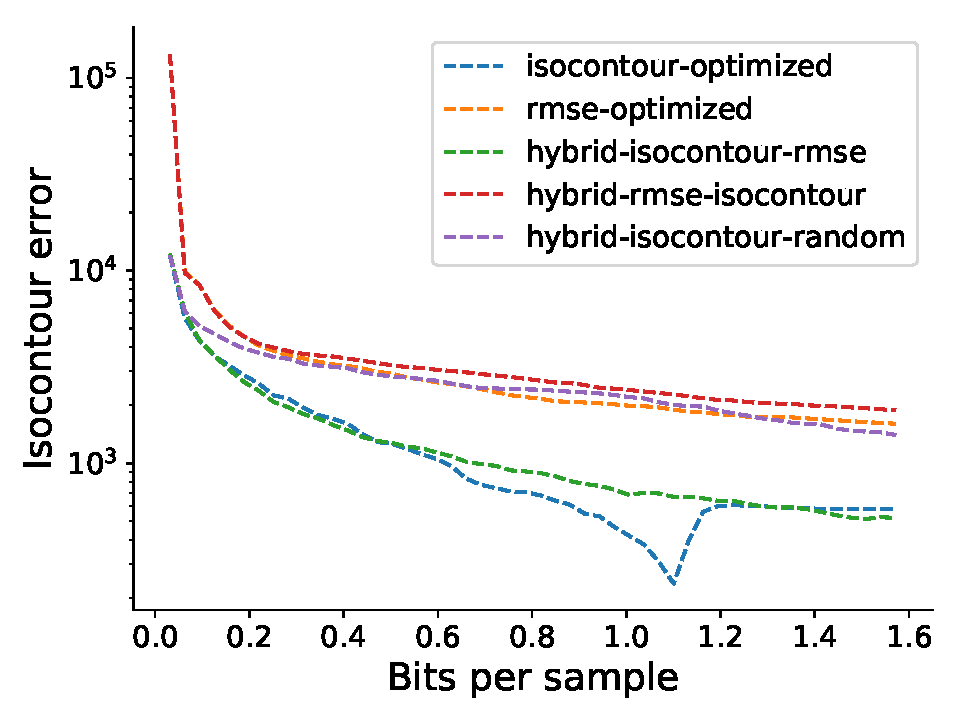
\includegraphics[width=0.48\linewidth]{img/isocontour/kingsnake-isocontour.pdf}}
	\subcaptionbox{kingsnake}
	{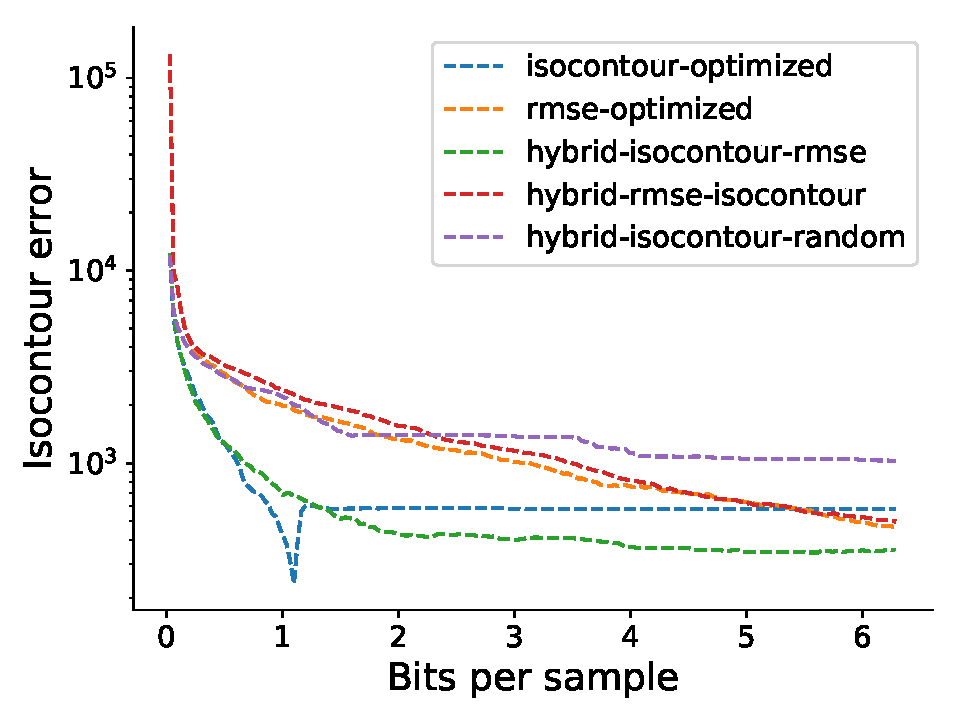
\includegraphics[width=0.48\linewidth]{img/isocontour/kingsnake-isocontour-long.pdf}}
	\subcaptionbox{pressure}
	{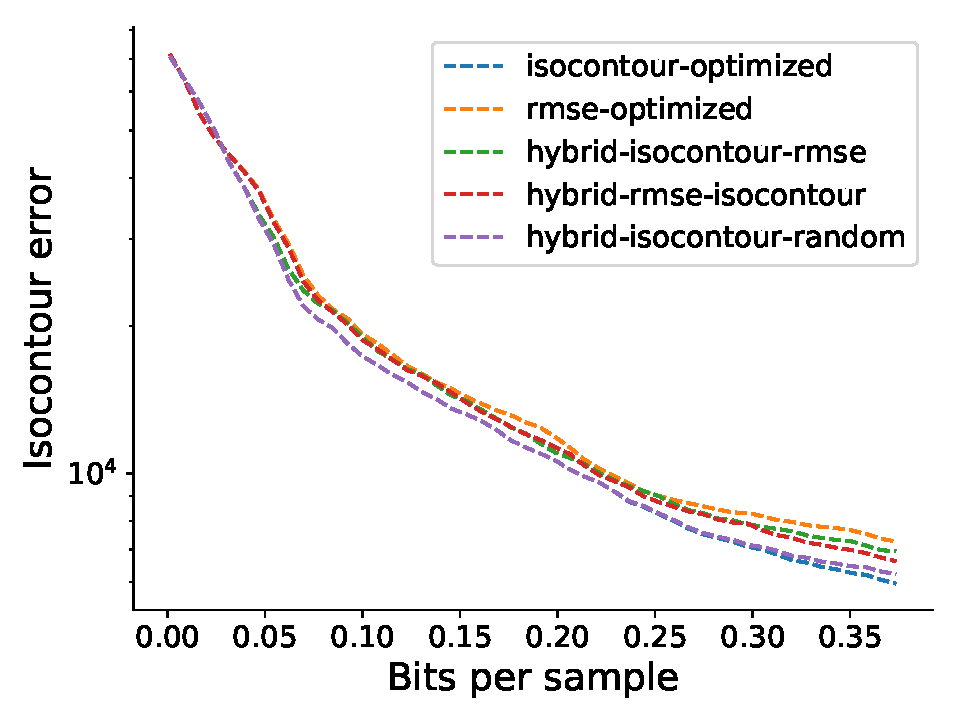
\includegraphics[width=0.48\linewidth]{img/isocontour/pressure-isocontour.pdf}}
	\subcaptionbox{viscosity}
	{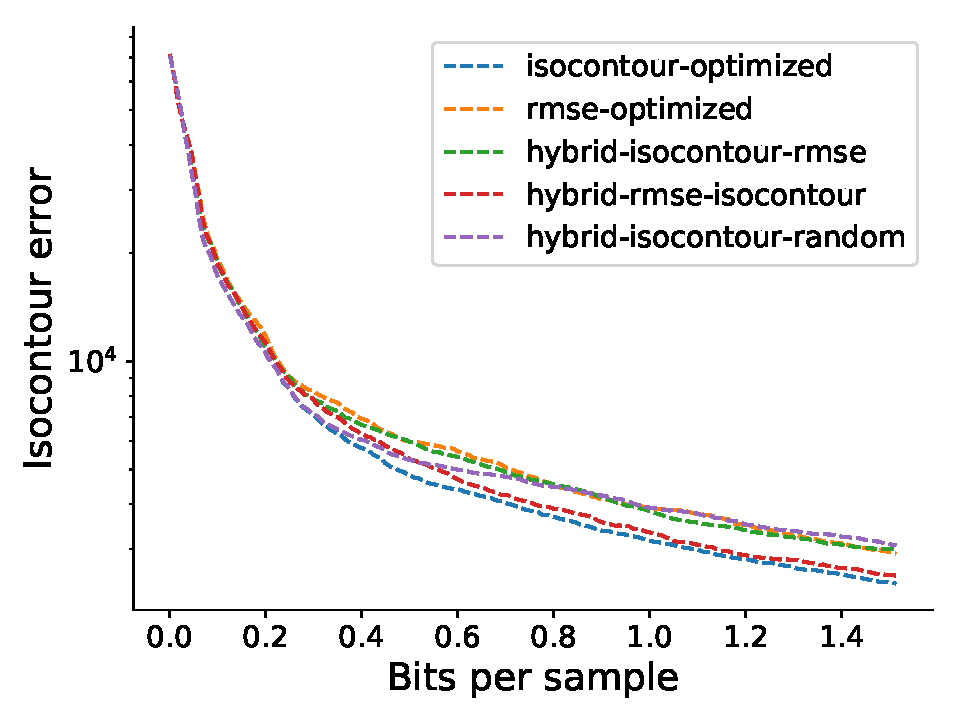
\includegraphics[width=0.48\linewidth]{img/isocontour/pressure-isocontour-long.pdf}}
	\subcaptionbox{viscosity}
	{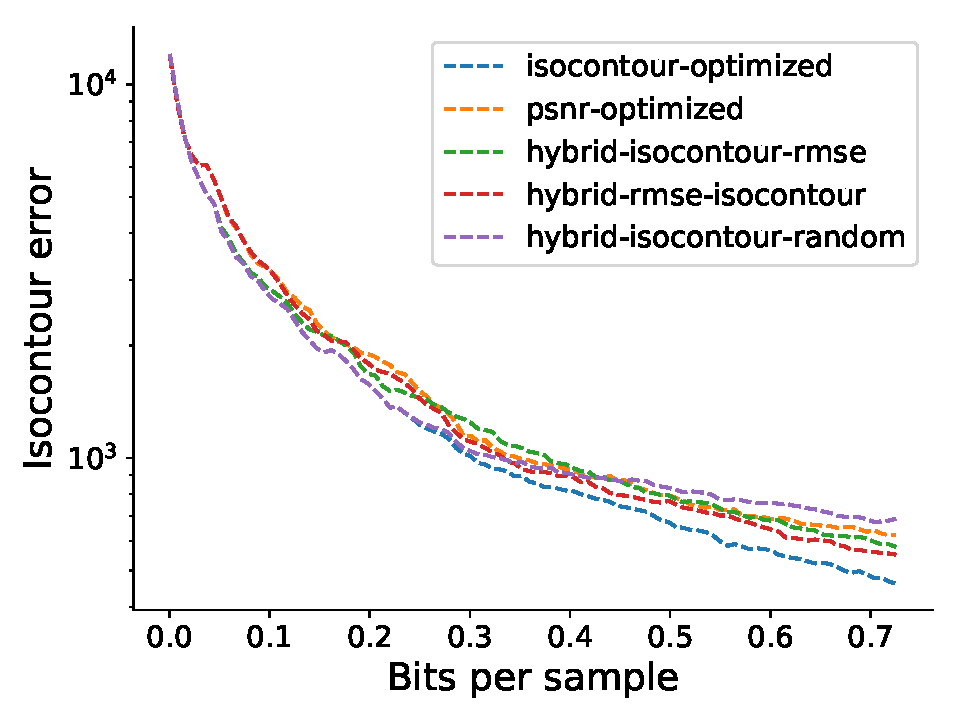
\includegraphics[width=0.48\linewidth]{img/isocontour/viscosity-isocontour.pdf}}
	\subcaptionbox{pressure}
	{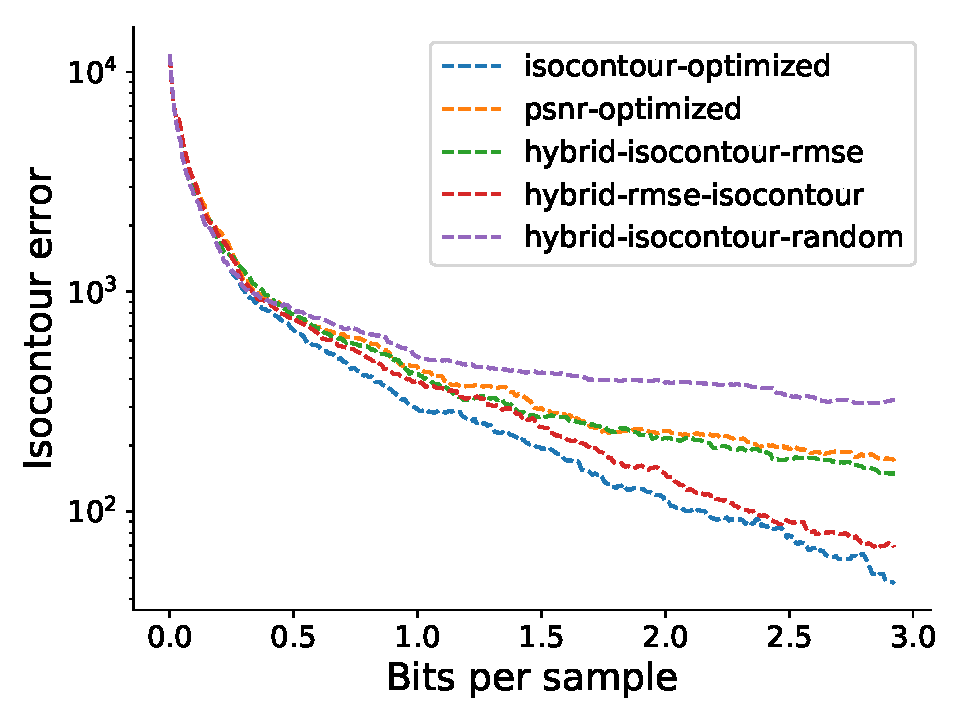
\includegraphics[width=0.48\linewidth]{img/isocontour/viscosity-isocontour-long.pdf}}
	\caption{Isocontour errors for \emph{rmse-optimized}, \emph{isocontour-optimized}, and their
	hybrid streams. The vertical axis is log-scaled. The bit rates are capped to highlight differences
	among streams.}
	\label{fig:isocontour-plots}
\end{figure}

The first thing to observe from Figure \ref{fig:isocontour-plots} is that the \emph{hybrid
isocontour-rmse} stream improves on \emph{rmse-optimized}, as expected. However, it underperforms
\emph{isocontour-optimized} by a considerable degree. This could be due to the fact that
\emph{hybrid isocontour-rmse} is more spatially adaptive to the contour, or that \emph{hybrid
isocontour-rmse} is fundamentally different than \emph{rmse-optimized}. To answer this question, we
form a special stream 

figure 3: show isocontour rendering for the three streams at some low bit rates where the errors are
apparent. Ideally the difference between isocontour and hybrid is not noticeable.

We argue that different isovalues will require different stream signatures, but thanks to the
similarity between hybrid and isocontour streams, the rmse stream can be used to extract isocontour
too, provided that it is paired with a method to localize the contour (e.g. min-max octrees etc).

Figure 5: We show that the hybrid and isocontour can diverge somewhat for low-gradient contour.
Valerio suggested here we coudl also build a "ramp" dataset at different angles and see if the two
diverges more as the ramp become flatter.

We argue that if the gradient is low, some noise bits at the end will make an impact, the isocontour
is very sensitive to noise, and is in general not interesting or meaninfgul to extract.
